\documentclass{article}
\newcommand{\BibTeX}{{\sc Bib}\TeX}
\newcommand{\ds}{\displaystyle}

%% The `ecrc' package must be called to make the CRC functionality available
\usepackage[table,xcdraw]{xcolor}
\usepackage[utf8x]{inputenc}
%\usepackage[latin1]{inputenc}
\usepackage[OT1]{fontenc}
\usepackage{pgf}

\usepackage{tikz}
\usepackage{gensymb}
\usepackage{subfigure}
\usepackage{caption2}
\usepackage[english]{babel}
\usepackage{amsmath}
\usepackage{graphicx}
%\usepackage[pdftex]{graphicx}
\usepackage{epstopdf}
\usepackage{fancyhdr}
\usepackage{subfigure}
\usepackage{psfrag}
%\usepackage{floatflt}   % pour floatingfigure
\usepackage{float}
%\usepackage{algorithm}
%\usepackage{algorithmic}
% The amssymb package provides various useful mathematical symbols
\usepackage{amssymb}
\usepackage{color}
\usepackage{xcolor}
\usepackage{geometry}
\usepackage{pict2e}
\usepackage{url}
\usepackage{multirow}
%\usepackage[table,xcdraw]{xcolor}


\usepackage{xcolor}
\usepackage{graphicx}
\usepackage{amsmath}
\usepackage{amsfonts}
\usepackage{amssymb}
\usepackage{multirow}

\usepackage{vhistory}

\graphicspath{ {./Figures/}}


\title {Solid mechanics equations for experiments}



\begin{document}
\maketitle
% Start of the revision history table
\begin{versionhistory}
  \vhEntry{1.0}{30.04.20}{B Bouscasse }{created}
%  \vhEntry{1.1}{23.01.04}{DP|JPW}{correction}
\end{versionhistory}

\section{Introduction}
This document aims to regroup the equations of mechanics traditionally used in experiments.  A notation is proposed. It also serves at support for the functions developped in Basin Tools project. 

\section{Example of a model}

The segmented hull model is presented in Figure \ref{figSegmentedHullModel}. 

%%%%%%%%%%%%%%%%%%%%%%%%%%%%%%%%
\begin{figure}[htbp]
\centering
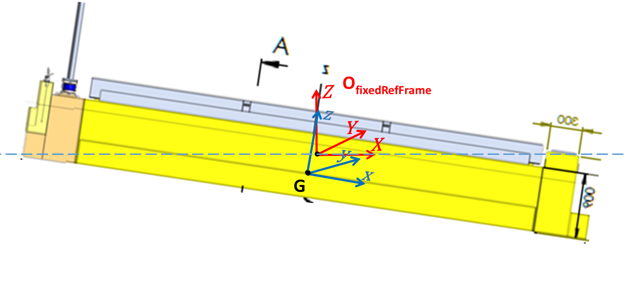
\includegraphics[width=0.8\textwidth]{BGF}
\caption{Sketch of the BGF platform}
\label{figSegmentedHullModel}
\end{figure}
%%%%%%%%%%%%%%%%%%%%%%%%%%%%%%%%




\section{Solid kinematics}

\subsection{Reference system}

The galilean reference system is given as $(O,\mathbf{x}_0, \mathbf{y}_0, \mathbf{z}_0)$, the body-fixed reference system $R_b$ is given as  $(O_b,\mathbf{x}, \mathbf{y}, \mathbf{z})$. The three rotations Yaw $\psi$, Pitch $\theta$  and Roll $\phi$ angles are Tait-Bryan angles.


\subsection{Vector notation}

The mathematical notation that allows to identify position, velocity and acceleration of different of points of interest of the mock-up must establish to express them in different frames. For instance, for a generic point of interest $P$ on the mock-up (the purpose of $P$ and $R_f (O_f,\mathbf{x_f}, \mathbf{y_f}, \mathbf{z_f})$ in this explanation are only use to described the sample notation):

\begin{enumerate}
	\item $\mathbf{r}_p^f$ denotes the position of $P$ with respect to a frame $R_f$: \\
	\begin{equation}\mathbf{r}_P^f = \mathbf{O_f P} \end{equation}
	\begin{equation}
	\mathbf{r}_P^f = x_P^f \mathbf{x}_f  + y_P^f \mathbf{x}_y + z_P^f \mathbf{x}_z \equiv \begin{bmatrix}
	x_P^f \\
	y_P^f \\
	z_P^f
	\end{bmatrix}
	= [x_P^f , y_P^f, z_P^f ]^T
	\end{equation}
	\item $\mathbf{v}_P^f$ denotes the velocity of $P$ with respect to a frame $R_f$.
	\\
	\begin{equation} \displaystyle \mathbf{v}_P^f = \mathbf{v}(P/R_f)  = \frac{d \mathbf{O_f P}}{dt}\Biggr\rvert_{R_f} \end{equation}
	
	\item $\dot{\mathbf{v}}_P^f$ denotes the acceleration of $P$ with respect to a frame $R_f$
	\item $ \mathbf{\Theta}_{0f}$ is vector of Euler angles Tait bryan that take the $R_0$ into the orientation of  $R_f$ 
	\item $\mathbf{\omega}_{0f}^f$ denotes the relative angular velocity of the $R_f$ with respect to $R_0$, decomposed in the $R_f$ \\
	An other notation could be $\mathbf{\omega}_{0f} = \mathbf{\omega}(R_f / R_0)$
\end{enumerate}

With those notations the 
\begin{equation} \displaystyle \mathbf{v}_P^f = \mathbf{v}(P/R_f)  = \frac{d \mathbf{O_f P}}{dt}\Biggr\rvert_{R_f} \end{equation}

The transformation of derivation basis is given with:
\begin{equation}
 \frac{d \mathbf{OP}}{dt}\Biggr\rvert_{R_0} =  \frac{d \mathbf{OP}}{dt}\Biggr\rvert_{R_f} + \mathbf{\omega}_{0f} \times  \mathbf{OP}
\end{equation}

If A and B are two points fixed with respect to the reference frame $R_f$ {\color{blue} what happens for moving point in f}
\begin{equation}
 \mathbf{v}_B^0 = \frac{d \mathbf{OB}}{dt}\Biggr\rvert_{R_0} =  \frac{d \mathbf{OA}}{dt}\Biggr\rvert_{R_0} + \mathbf{\omega}_{0f} \times  \mathbf{AB}
\end{equation}

\subsection{Rotations}

The mock-up attitude orientation is defined by the orientation of the body-fixed reference system $R_b$ relative to $R_0$. This is given by three instrinsic rotations that take the $R_0$ into $R_b$ defined by three angles roll $\phi $,  pitch $\theta$, and yaw $\psi$.
These rotations are called Tait-Bryan angles or Euler angles defined as: 

\begin{equation}
\mathbf{\Theta}_{0b} \stackrel{\Delta}{=} 
\begin{bmatrix}
\psi \\
\theta \\
\phi
\end{bmatrix} 
\end{equation}


The vector coordinates between different frames can be transform via appropriate matrices. Following \cite{perez2005ship}, the generic vector $\textbf{t}$ can be address either in frame $0$ or the frame $b$ as:

\begin{equation}
	\textbf{t}= \begin{bmatrix}
	x_{t}^0 \\
	y_{t}^0\\
	z_{t}^0
	\end{bmatrix}^0 
=  \begin{bmatrix}
	x_{t}^b \\
	y_{t}^b\\
	z_{t}^b
	\end{bmatrix}^b
\end{equation}


This lead to the transformation matrix with notation $ R_{b0}  \stackrel{\Delta}{=}  R_{b0} (\mathbf{\Theta}_{0b})$, which can be expressed in the $b$-frame to the $0$-frame as:

\begin{equation}\label{vectortransform}
\textbf{t}^0 =  R_{b0} \cdot\textbf{t}^b
\end{equation}

where the rotation matrix $ R_{b0} $ is obtained with three consecutive rotations about the successive axes obtained during intrisic rotations:

\begin{equation}
 R_{0b} \stackrel{\Delta}{=} 
\textbf{R}_{x_b,\phi} \: \textbf{R}_{y',\theta} \: \textbf{R}_{z_0,\psi}
\end{equation}
Where \cite{perez2005ship}, 

\begin{equation}
\textbf{R}_{x_b,\phi} = 
\begin{bmatrix}
1 & 0 & 0 \\
0 & \cos \phi &-\sin \phi \\
0 & \sin \phi & \cos \phi
\end{bmatrix}, \quad
\textbf{R}_{y',\theta} =
\begin{bmatrix}
\cos \theta & 0 & \sin \theta \\
0 & 1 & 0 \\
-\sin \theta & 0 & \cos \theta
\end{bmatrix}, \quad
\textbf{R}_{z_0,\psi} =
\begin{bmatrix}
\cos \psi & -\sin \psi & 0 \\
\sin \psi & \cos \psi & 0 \\
0 & 0 & 1
\end{bmatrix}
\end{equation}

\begin{equation}
 R_{b0}  =
\begin{bmatrix}
\cos \psi \cos \theta & -\sin \psi \cos \phi + \cos \psi \sin \theta \sin \phi & \sin \psi \sin \phi + \cos \psi \cos \phi \sin \theta \\
\sin \psi \cos \theta & \cos \psi \cos \phi + \sin \phi \sin \theta \sin \psi & -\cos \psi \sin \phi + \sin \phi \cos \phi \sin \theta \\
- \sin \theta & \cos \theta \sin \phi & \cos \theta \cos \phi
\end{bmatrix}
\end{equation}


And, 

\begin{equation}
 R_{b0} =  R_{0b}^{-1} =R_{0b}^{T}
\end{equation} \label{}

The transformation of velocities $\mathbf{v^b_{O_b}}=(u,v,w)$ of origin of expressed in $R_b$  and $\mathbf{v^0_{O_b}}$ the time derivative of the position in $R_0$  can be expressed as:

\begin{equation}
\begin{bmatrix}
\dot{x_{O_b}} \\
\dot{y_{O_b}} \\
\dot{z_{O_b}}
\end{bmatrix}^0 
=
 R_{b0} 
\begin{bmatrix}
u \\
v \\
w
\end{bmatrix}^b 
\end{equation}


The vector of angular velocity $\mathbf{\omega}_{0b}^b$ in the fixed body frame, $b$-frame related to the time rate of change of the Euler angles $\mathbf{\Theta}_{0b}$ can be expressed as:

\begin{equation}
\dot{\mathbf{\Theta}}_{0b} = \mathbf{T}_{b0} \,  \mathbf{\omega}_{0b}^b,
\quad \text{or}
\begin{bmatrix}
\dot{\phi} \\
\dot{\theta} \\
\dot{\psi}
\end{bmatrix} 
=  T_{b0}
\begin{bmatrix}
p \\
q \\
r
\end{bmatrix} 
\end{equation}\

The notation  $\mathbf{T}_{b0}$ has to be understood that it transformsan angular velocity expressed clearly in $R_b$ in a velocity expressed in the construction basis so ``b0''.

The transformation matrix $\textbf{T}_{\Theta} (\mathbf{\Theta}_{0b})$ can be derived from \cite{Fossen}:

\begin{equation}
\mathbf{\omega}_{0b}^b =
\begin{bmatrix}
p \\
q  \\
r
\end{bmatrix}
=
\begin{bmatrix}
\dot{\phi} \\
0  \\
0
\end{bmatrix}
+ \textbf{R}_{x_b,\phi}^T
\begin{bmatrix}
0 \\
\dot{\theta}  \\
0
\end{bmatrix}
+ \textbf{R}_{x_b,\phi}^T \:\textbf{R}_{y',\theta}^T
\begin{bmatrix}
0 \\
0  \\
\dot{\psi}
\end{bmatrix}
\stackrel{\Delta}{=}
\textbf{T}_{0b} \dot{\mathbf{\Theta}}_{0b}
\end{equation}

Where $\mathbf{T}_{b0}$ is the transformation matrix and its inverse given by:

\begin{equation}
\textbf{T}_{b0} =
\begin{bmatrix}
1 & \sin \phi \tan \theta & \cos \phi \tan \theta \\
0 & \cos \phi & -\sin \phi  \\
0 & \sin \phi / \cos \theta & \cos \phi / \cos \theta
\end{bmatrix}, 
\quad
\textbf{T}_{0b} =
\begin{bmatrix}
1 & 0 & - \sin \theta \\
0 & \cos \phi & \cos \theta \sin \phi  \\
0 & -\sin \phi & \cos \phi \cos \theta
\end{bmatrix}
\end{equation}


{\color{blue} 
\subsubsection{I don't know where this goes}

Therefore, the position orientation vector is defined as:

\begin{equation}
\mathbf{\eta} \stackrel{\Delta}{=} 
\begin{bmatrix}
\textbf{r}_{O_b}^0 \\
\mathbf{\Theta}_{0b}
\end{bmatrix} 
=
[x_G,y_G,z_G,\psi,\theta,\phi]^T
\end{equation}

While the linear and angular velocity vector of the body are conveniently expressed in $b$-frame as:

\begin{equation}
\mathbf{\nu} \stackrel{\Delta}{=} 
\begin{bmatrix}
\textbf{v}_G^b \\
\mathbf{\omega}_{0b}^b
\end{bmatrix} 
=
[u,v,w,p,q,r]^T
\label{velocityvector}
\end{equation}

Where $\textbf{v}_{G}^b = [u,v,w]^T$ is the linear velocity of the point $G$ expressed in the $b$-frame, and $\mathbf{\omega}_{0b}^b = [p,q,r]^T$ is the angular velocity of the $b$-frame with respect to $0$-frame expressed in the $b$-frame.
Expression of p, q, r is detailed in the next section.

The velocity $\textbf{v}^0$ of any point of the solid in the galilean frame is expressed with:
\begin{equation}
\textbf{v}^0 = \textbf{v}_G^0  +   \mathbf{\omega}_{0b}^b \times \textbf{r}^b
\end{equation} 
}

\subsection{Velocity transformations}


\subsubsection{Definitions}
The movement of a solid `b' with respect to a reference frame  $R_0$ defined by the set of rotations $R_{b0}$ and translations $\textbf{d}(t)$ assembled into the homogeneous transformation $[T(t)]=[ R_{b0} (t) \,  \textbf{d}(t) ]$.  

$ \textbf{d}(t)$ corresponds to {\color{blue} the  position of the origin of the moving frame in $R_0$ }. $\mathbf{v}^0_{O_b}=\dot{\textbf{d}}$ and $\mathbf{a}^0_{O_b} = \ddot{\textbf{d}}$ are respectively the velocity and the acceleration of  the origin $O_b$ of the moving frame  $R_b$.



\subsubsection{Position}
If  $\mathbf{r^b_P}$' are the coordinates of a point ''P'' attached to the solid body measured in the moving reference frame $R_b$, then the trajectory of this point traced in $R_0$' is given by:
\begin{equation} \mathbf{r^0_P}(t)=[T(t)]\mathbf{r^b_P}(t)
\end{equation}

It is convenient to expand T in the following way.
\begin{equation}
\begin{bmatrix} \mathbf{r^0_P} \\ 1\end{bmatrix}=\begin{bmatrix}  R_{b0} & \textbf{d} \\ 0 & 1\end{bmatrix}
\begin{bmatrix} \mathbf{r^b_P} \\ 1\end{bmatrix}.\end{equation}


This equation for the trajectory of ''P'' can be inverted to compute the coordinate vector '''p''' in  $R_b$ as:
\begin{equation} \mathbf{r^b_P} = [T(t)]^{-1}\mathbf{r^0_P} \end{equation}

\begin{equation} 
\begin{bmatrix} \mathbf{r^b_P} \\ 1\end{bmatrix}=\begin{bmatrix} R_{b0}^T & -R_{b0}^T\textbf{d} \\ 0 & 1\end{bmatrix}
\begin{bmatrix} \mathbf{r^0_P} \\ 1\end{bmatrix}.\end{equation}
This expression uses the fact that the transpose of a rotation matrix is also its inverse, that is:
\begin{equation} R_{b0}^T \,R_{b0}=I.\!\end{equation}

\subsubsection{Velocity}
The velocity of the point ''P'' along its trajectory '''P'''(t) is obtained as the time derivative of this position vector
\begin{equation} \mathbf{v}^0_P = [\dot{T}(t)]\mathbf{r^b_P} \end{equation}

\begin{equation} 
\begin{bmatrix}  \mathbf{v}^0_P  \\ 0\end{bmatrix} = \frac{d}{dt} {\begin{bmatrix} R_{b0} & \textbf{d}(t) \\ 0 & 1 \end{bmatrix}}
\begin{bmatrix} \mathbf{r^b_P} \\ 1\end{bmatrix} = \begin{bmatrix} \dot{R_{b0}} & \dot{\textbf{d}}(t) \\ 0 & 0 \end{bmatrix}
\begin{bmatrix} \mathbf{r^b_P} \\ 1\end{bmatrix}.\end{equation}

{\color{blue} This would mean $\frac{d\mathbf{r^b_P}}{dt} = 0$ so that means P is fixed in $R_b$
The dot denotes the derivative with respect to time; because '''p''' is constant, its derivative is zero.
}
\begin{equation}
\mathbf{v^0_P}  =  [\dot{T}(t)][T(t)]^{-1}\mathbf{r^0_P}(t)
\end{equation}
 
 
 \begin{equation}
\begin{bmatrix} \mathbf{v^0_P} \\ 0\end{bmatrix} = \\
\begin{array}{l}
\begin{bmatrix} \dot{R_{b0}} & \dot{\textbf{d}} \\ 0 & 0 \end{bmatrix}
\begin{bmatrix} R_{b0} & \textbf{d} \\ 0 & 1 \end{bmatrix}^{-1}
\begin{bmatrix} \mathbf{r^0_P}(t) \\ 1\end{bmatrix}  = \\
\begin{bmatrix} \dot{R_{b0}} & \dot{\textbf{d}} \\ 0 & 0 \end{bmatrix}
R^{-1}\begin{bmatrix} 1 & -\textbf{d} \\ 0 & R_{b0} \end{bmatrix}
\begin{bmatrix} \mathbf{r^0_P}(t) \\ 1\end{bmatrix}  = \\
\begin{bmatrix} \dot{R_{b0}}R_{b0}^{-1} & -\dot{R_{b0}}R_{b0}^{-1}\textbf{d} + \dot{\textbf{d}} \\ 0 & 0 \end{bmatrix}
\begin{bmatrix} \mathbf{r^0_P}(t) \\ 1\end{bmatrix}  = \\
\begin{bmatrix} \dot{R_{b0}}R_{b0}^T & -\dot{R_{b0}}R_{b0}^T\textbf{d} + \dot{\textbf{d}} \\ 0 & 0 \end{bmatrix}
\begin{bmatrix} \mathbf{r^0_P}(t) \\ 1\end{bmatrix} 
\end{array}
\end{equation}
 
 \begin{equation}
\mathbf{v^0_P}  = [S]\mathbf{r^0_P}.
\end{equation}

The matrix [S] is given by:
\begin{equation} [S] =  \begin{bmatrix} \Omega & -\Omega\textbf{d} + \dot{\textbf{d}} \\ 0 & 0 \end{bmatrix}\end{equation}
where
\begin{equation} [\Omega] = \dot{R_{b0}}R_{b0}^T,\end{equation}
is the angular velocity matrix.

Multiplying by the operator [S], the formula for the velocity $\mathbf{v^0_P}$ takes the form:
\begin{equation}\mathbf{v^0_P} = \Omega (\mathbf{r^0_P}-\textbf{d}) + \dot{\textbf{d}} =  \mathbf{\omega}_{0b} \times  \mathbf{r^b_P} + \mathbf{v}^0_{O_b},\end{equation}
where the vector $ \mathbf{\omega}_{0b}$ is the angular velocity vector obtained from the components of the matrix  $\Omega$; the vector
\begin{equation}  \mathbf{r^P}_{R_b} =\mathbf{r^0_P}-\textbf{d},\end{equation}
is the position of ''P'' relative to the origin ''O'' of the moving frame $R_b$.


\subsubsection{Acceleration}
The acceleration of a point ''P'' in a moving body ''B'' is obtained as the time derivative of its velocity vector:
\begin{equation}\mathbf{a}^0_P = \frac{d}{dt}\mathbf{v^0_P} = \frac{d}{dt}\big([S]\mathbf{r^0_P}\big)=[\dot{S}]\mathbf{r^0_P} + [S]\dot{\mathbf{r^0_P}} = [\dot{S}]\mathbf{r^0_P} + [S][S]\mathbf{r^0_P} .\end{equation}

This equation can be expanded firstly by computing
\begin{equation} [\dot{S}] =  \begin{bmatrix} \dot{\Omega} & -\dot{\Omega}\textbf{d}  -\Omega\dot{\textbf{d}}  + \ddot{\textbf{d}} \\ 0 & 0 \end{bmatrix} = \begin{bmatrix} \dot{\Omega} & -\dot{\Omega}\textbf{d}  -\Omega \mathbf{v}^0_{O_b}  + \mathbf{a}^0_{O_b} \\ 0 & 0 \end{bmatrix}\end{equation}
and
\begin{equation} [S]^2 =  \begin{bmatrix} \Omega & -\Omega\textbf{d} + \mathbf{v}^0_{O_b}  \\ 0 & 0 \end{bmatrix}^2 = \begin{bmatrix} \Omega^2 & -\Omega^2\textbf{d} + \Omega \mathbf{v}^0_{O_b}  \\ 0 & 0 \end{bmatrix}.\end{equation}

The formula for the acceleration  $\textbf{A}_P$ can now be obtained as:
\begin{equation} \mathbf{a}^0_P= \dot{\Omega}(\mathbf{r^0_P} - \textbf{d})  + \mathbf{a}^0_{O_b} + \Omega^2(\mathbf{r^0_P}-\textbf{d}),\end{equation}
or
\begin{equation} \mathbf{a}^0_P = \mathbf{a}^0_{O_b} + \frac{d \mathbf{ \omega}_{0b}}{dt}  \times  \mathbf{r^P}_{R_b} + \mathbf{ \omega}_{0b} \times \mathbf{ \omega}_{0b} \times \mathbf{r^P}_{R_b} ,\end{equation}
where $\frac{d \, \mathbf{ \omega}_{0b}}{dt}$ is the angular acceleration vector obtained from the derivative of the angular velocity matrix;








\subsection{Newton/Euler equation of motion on a moving frame}

The 6DOF motions of a generic body are computed by solving the standard Euler law in the body-fixed reference frame $R_b$ with the origin O not coinciding with the center of gravity G, which position is defined by the vector  $\mathbf{r^G}$  (\cite{fossen2011handbook}):
\begin{equation}
\label{eq:7}
\begin{array}{lll}
\ds m \left( \frac{d\mathbf{V}_{R_b}}{dt}+\mathbf{\Omega}_{R_b} \times \mathbf{V}_{R_b} +\frac{ d\mathbf{\Omega}_{R_b}}{dt} \times  \mathbf{r^G}_{R_b}  + \mathbf{\Omega}_{R_b} \times (\mathbf{ \Omega}_{R_b} \times  \mathbf{r^G}_{R_b})   \right) = \mathbf{F}_{R_b}
\\[0.5cm]
\ds I\frac{d\mathbf{\Omega}_{R_b}}{dt}+\mathbf{\Omega}_{R_b} \times I\mathbf{\Omega}_{R_b} + m \mathbf{r^G}_{R_b} \times \left( \frac{d\mathbf{V}_{R_b}}{dt} + \mathbf{\Omega}_{R_b} \times \mathbf{V}_{R_b}  \right)=\mathbf{M}_{R_b}
\end{array}
\end{equation}

where $m$ and $I$ are the mass and moments of inertia tensor of the hull, respectively. $\mathbf{V}_{R_b}=(u,v,w)^T$ at the origin O and $\mathbf{\Omega}_{R_b}=(p,q,r)^T$ are the vectors of translational ( surge, sway, heave) and angular velocities (roll, pitch, yaw). $\mathbf{F}^{ext}_{Rb}=(F_x, F_y, F_z)^T$ and $\mathbf{M}^{ext}_{Rb}=(M_x, M_y, M_z)^T$ are the vectors of  force and moment with respect to O acting on the body. $\mathbf{r}_{R_b}^{G} = (x_G, y_G, z_G)$ is the position of the center of gravity G in the body fixed coordinate system. Note that the superscript $T$ denotes the transpose of a vector or a matrix.
 $\mathbf{F}^{ext}_{Rb}$ and $\mathbf{M}^{ext}_{Rb}$ represents the hydrostatic and hydrodynamic forces and moments together with the weight.






\subsection{Relation between the load balance measurements in segments and shear stress and bending moments}
\label{FHydro}
With the experimental setup used the ATI balance measures directly the shear force and the bending moment at the intersegment 4. However, the load balances $c_i$ installed on each segment between the beam $b_i$ and the hull segment $h_i$ (see Figure \ref{figSegmentedHullSketch} ) at the position $O_i$ $(x_{si},0,z_{si})$ does not directly measure the external hydrodynamic and hydrostatic forces and moments acting on this segment. 
For each segment, the application of Euler/Newton equation of motion (Eq. \ref{eq:7}) on $h_i$ which is everything below the sensor (and contain the hull) gives:
\begin{equation}
\begin{array}{l}
\displaystyle  m_{h_i} (\frac{d\mathbf{V_{h_i}}}{dt}+\mathbf{\Omega} \times \mathbf{V_{h_i}})   =  \mathbf{P}_{h_i} +  \mathbf{F}_{hydro/h_i}  +  \mathbf{F}_{c_i/h_i} \, \, \text{ for each segment} \, i  \\
\displaystyle  I_{h_i}\frac{d\mathbf{\Omega}}{dt}+\mathbf{\Omega} \times  I_{h_i}\mathbf{\Omega} =  \mathbf{M}_{P_{h_i}} +  \mathbf{M}_{hydro/h_i}  +  \mathbf{M}^{G_h}_{c_i/h_i} \, \, \text{ for each segment} \, i
\end{array}
\end{equation}
where $m_{h_i}$ and $I_{h_i}$ are mass and inertia tensor for $h_i$, $\mathbf{P}_{h_i}$ and  $\mathbf{M}_{P_{h_i}}$ are the weight and the moment exerted by the weight in $O_i$, $\mathbf{F}_{hydro/h_i}$ and  $\mathbf{M}_{hydro/h_i}$ the hydrodynamic force and moments. 
 $\mathbf{F}_{c_i/h_i}$ and $\mathbf{M}^{G_h}_{c_i/h_i}$  are related to the measurement on the sensor $\mathbf{T}_{c_i}$  defined as:
\begin{equation}
\begin{array}{l}
\mathbf{F}_{c_i/b_i}   = - \mathbf{F}_{c_i/h_i} = \mathbf{T}_{c_i} = T_{c_i} \mathbf{z} \\
 \mathbf{M}_{c_i/b_i}   = - \mathbf{M}^{O_i}_{c_i/h_i} = \mathbf{R}_{c_i} = R^y_{c_i} \mathbf{y} + R^x_{c_i} \mathbf{x}
\end{array}
\end{equation}
with 
\begin{equation}
\mathbf{M}^{G_h}_{c_i/h_i}  = \mathbf{M}^{O_i}_{c_i/h_i} + \mathbf{G_h O_i} \times  \mathbf{F}_{c_i/h_i} 
\end{equation}

This leads to the formulation of hydrodynamic forces and moments acting on each segment:
\begin{equation}
\begin{array}{l}
\displaystyle \mathbf{F}_{hydro/h_i}  = m_{h_i} (\frac{d\mathbf{V_{h_i}}}{dt}+\mathbf{\Omega} \times \mathbf{V_{h_i}}) -  \mathbf{P}_{h_i}  + \mathbf{T}_{c_i}  \\
\displaystyle  \mathbf{M}_{hydro/h_i} =  I_{h_i}\frac{d\mathbf{\Omega}}{dt}+\mathbf{\Omega} \times  I_{h_i}\mathbf{\Omega}  +  \mathbf{R}_{c_i} - \mathbf{M}_{P_{h_i}}
\end{array}
\end{equation}






\subsection{Linear momentum}

General definition of momentum $\mathbf{r^b_P}$ of the solid $R$ is given as:
\begin{equation}
\mathbf{r^b_P} = \int_{R} \textbf{v}^0 \: \text{dm}
\end{equation}
where $ \textbf{v} ^0$ is the velocity of the elementary element $\text{dm}$ in the galilean reference frame.
The momentum at the center of gravity can be establish as:

\begin{align} 
\mathbf{r^b_P} &= \int_{R} \textbf{v}\: \text{dm} \\
& = \int_{R} \frac{d \: \textbf{r}^0}{dt} \:  \text{dm}\\ \label{MomentumTemp}
& =  \frac{d}{dt} \bigg( \int_{R} \textbf{r}^0 \:  \text{dm}  \bigg) \\ 
& = \frac{d}{dt} (m \: \textbf{r}_G^0) \\
&= m \textbf{v}_G^0 \label{Momentum}
\end{align}

Noticed that the time derivative in is put outside the integral whose region of integration $R$ depend on time. This manipulation is justified because center of gravity of rigid body behaves as material point as explained in \cite{Oliver,Casey}. 


\subsection{Angular momentum and moment of inertia}

The angular momentum of a rigid body relative to its center of gravity and the fixed origin of the reference 0-frame $0$ are denoted respectively as $\textbf{h}$ and $\textbf{H}_0$. By definition:



% H is sigma p104 Le Houedec
\begin{equation}
\textbf{h}= \int_{R} \textbf{r}^b \times \textbf{v}^0 \:  \text{dm},
\quad
\textbf{h}_0= \int_{R} \textbf{r}^0 \times \textbf{v}^0\: \text{dm}
\end{equation}


Expending the angular momentum $\textbf{H}$:

\begin{align}\label{angularmomentum}
\textbf{h} &= \int_{R} \textbf{r}^b \times (\textbf{v}_G^0  +   \mathbf{\omega}_{0b}^b \times \textbf{r}^b) \:  \text{dm}, \\
    & = \int_{R} \textbf{r}^b \times \textbf{v}_G^0  \:  \text{dm}   +  \int_{R}  \textbf{r}^b \times  (\mathbf{\omega}_{0b}^b \times \textbf{r}^b) \:  \text{dm}, \\
  & =  \int_{R}  \textbf{r}^b \times  (\mathbf{\omega}_{0b}^b \times \textbf{r}^b) \:  \text{dm}, 
\end{align}


Expending the angular momentum $\textbf{h}_0$ \textcolor{red}{Check}:

\begin{align}
\textbf{h}_0 & = \int_{R} \textbf{r}^0 \times \textbf{v}^0\: \text{dm} \\
 & = \int_{R} (\textbf{r}_G^0 + \textbf{r}^b)  \times \textbf{v}^0\: \text{dm} \\
& =  \textbf{h} +   \textbf{r}_G^0  \times \mathbf{r^b_P}
%\textbf{H} &= \int_{R} \textbf{r}^b \times \textbf{v} \: \rho \text{dv} \\
%& = \int_{R}  \textbf{r}^b \times (\textbf{v}_G^b + \mathbf{\omega}_{Ob}^b(\textbf{r}^b))  \: \rho \text{dv}  \\
%& = \int_{R}  \textbf{r}^b \times \textbf{v}_G^b  \: \rho \text{dv} + \int_{R} \textbf{r}^b (\mathbf{\omega}_{Ob}^b \cdot \textbf{r}^b) \: \rho \text{dv} \label{angularmomentum}
\end{align}


 Equation \ref{angularmomentum} can also be rewritten as: 

\begin{equation} \label{angularmomentumFinal}
\textbf{h}=  \int_{R} \textbf{r}^b \times (\mathbf{\omega}_{0b}^b \times \textbf{r}^b) \: \text{dm} =  \int_{R} ((\textbf{r}^b\cdot \textbf{r}^b) \mathbf{\omega}_{0b}^b - (\textbf{r}^b\cdot \mathbf{\omega}_{0b}^b)\textbf{r}^b) \: \text{dm}
\end{equation}

Using 
\begin{equation}
	\textbf{r}^b=
  \begin{bmatrix}
	x_{b} \\
	y_{b} \\
	z_{b}
	\end{bmatrix}^b
\end{equation}

the expression can be developped in
\begin{align} \label{angularmomentumtoInertia}
\textbf{h} & =    \mathbf{\omega}_{0b}^b \int_{R} ({x_{b}}^2 + {y_{b}}^2 + {z_{b}}^2 ) \: \text{dm}  + \int_{R} \textbf{r}^b ({x_{b}} p + {y_{b}} q + {z_{b}} r)  \: \text{dm} \\
& = \int_{R}
\begin{bmatrix}
(y_b^2 + z_b^2)  &  - x_b y_b & - x_b z_b \\
 - x_b z_b & (x_b^2 + z_b^2) & -y_b z_b\\
 - x_b z_b &  -y_b z_b & (x_b^2 +y_b^2)
\end{bmatrix}\,  \mathbf{\omega}_{0b}^b
\end{align}

where the matrix of inertia with respect to the center of gravity $\textbf{I}^b_g$ appears:
\begin{equation}
 \textbf{h}=   \textbf{I}^b_g \, \,  \mathbf{\omega}_{0b}^b
\end{equation}


\section{Newton/Euler 2nd law}

% write 3.15 from Fossen
The motions of the mock-up in 3 DOF therefore are computed by solving the standard Euler's law in the $b$-frame with the $G$ coinciding with the COG:  

\begin{align}
	\frac{d \mathbf{r^b_P}}{dt} =  & m(\frac{d \: \textbf{v}_{G}^b}{dt} + \mathbf{\omega}_{0b}^b \times \textbf{v}_{G}^b) = \textbf{F}_b \\
	\frac{d \textbf{h}}{dt} = & \textbf{I}^b_g(\frac{d \: \mathbf{\omega}_{0b}^b }{dt} + \mathbf{\omega}_{0b}^b \times \textbf{I}^b_g \: \textbf{v}_{G}^b) = \textbf{M}_b
\end{align}

Where $m$ is the mass and moments of inertia $I$ of the mock-up defined as:


 $\textbf{F}_b = (F_x, F_y, F_z)$ and  $\textbf{M}_b = (Mx, My, M_z)$ are the vectors of force and moment acting on the mock-up. 

\section{Energy conservation}
The definition of the kinetic energy is given by 
\begin{equation} \label{kineticgeneric}
E_k = \frac{1}{2} \int_{R} \textbf{v}^2  \text{dm} 
\end{equation}
it becomes with the previous definitions:
\begin{align} 
E_k &= \frac{1}{2} m \textbf{v}_G^b \cdot \textbf{v}_G^b +  \frac{1}{2}  {\omega}_{0b}^b \cdot \textbf{I}^b_g  \mathbf{\omega}_{0b}^b  
\end{align}


%
\section{Other writing to compare}
Here applied on mass over the balance

\begin{equation}
\begin{array}{l}
\displaystyle m \mathbf{a}^0_G = m \mathbf{g} + \mathbf{F}_{ext} - \mathbf{F}_m \\
\displaystyle \mathbf{M^B} = \mathbf{M^B_{P_m}}+\mathbf{M^B_{F_{ext}}}+ \mathbf{M^B_{-F_{m}}} 
\end{array}
\end{equation}

\begin{equation}\label{momentdynamique}
\mathbf{M^B} = \int_{\text{body}} \mathbf{BM}\times \mathbf{a}^0_M dm 
\end{equation}

\begin{equation} \mathbf{a}^0_M = \mathbf{a}^0_{G} + \frac{d \mathbf{ \omega}_{0b}}{dt}  \times  \mathbf{GM} + \mathbf{ \omega}_{0b} \times ( \mathbf{ \omega}_{0b} \times \mathbf{GM}) ,\end{equation}

As $\mathbf{ \omega}_{0b}$ and  $\mathbf{a}^0_{G}$ do not depend on the point M, and introducing the inertia operator around G $\mathbf{I_G}$ as:

\begin{equation}
\mathbf{I_G} \, \mathbf{X} =  \int_{\text{body}}  \mathbf{GM} \times (\mathbf{X} \times  \mathbf{GM}) dm 
\end{equation}
 
The relation \ref{momentdynamique} can be rewritten in:
 \begin{equation}
 \mathbf{M^B} =\mathbf{BM}\times m \mathbf{a}^0_{G} + \mathbf{I_G} \frac{d \mathbf{ \omega}_{0b}}{dt} +  \int_{\text{body}} \mathbf{GM}\times  \mathbf{ \omega}_{0b} \times (\mathbf{\omega}_{0b} \times \mathbf{GM} ) dm 
\end{equation}

\begin{equation}
\begin{array}{ll}
 \int_{\text{body}} \mathbf{GM}\times  \mathbf{ \omega}_{0b} \times (\mathbf{\omega}_{0b} \times \mathbf{GM} ) dm  &= -  \int_{\text{body}} \mathbf{GM}\times  (\mathbf{ \omega}_{0b} \times  \mathbf{GM} )  \times \mathbf{\omega}_{0b} dm  \\
 &= \mathbf{\omega}_{0b} \times \mathbf{I_G} \,  \mathbf{\omega}_{0b}
\end{array}
\end{equation}

The final expression for $ \mathbf{M^B}$ is
 \begin{equation}
 \mathbf{M^B} =\mathbf{BM}\times m \mathbf{a}^0_{G} + \mathbf{I_G} \frac{d \mathbf{ \omega}_{0b}}{dt} +   \mathbf{\omega}_{0b} \times \mathbf{I_G} \,  \mathbf{\omega}_{0b} 
\end{equation}



 \begin{equation}
\mathbf{M^B_{F_{ext}}} = \mathbf{BM}\times m \mathbf{a}^0_{G} + \mathbf{I_G} \frac{d \mathbf{ \omega}_{0b}}{dt} +   \mathbf{\omega}_{0b} \times \mathbf{I_G} \,  \mathbf{\omega}_{0b}  - \mathbf{M^B_{P_m}} - \mathbf{M^B_{-F_{m}}}  
\end{equation}

\section{Accelerometers}
An accelerometer measures $\mathbf{a} -\mathbf{g}$ in the fixed body coordinates. 

\section{Gyroscopes}
Gyroscopes should be able to measure $\mathbf{ \omega}_{0b}$


\section{Other things}
\subsection{Instantaneous centre of rotation}

\begin{equation}
\mathbf{V_A} =\mathbf{V_B} + \mathbf{A B} \times  \mathbf{\omega}_{0b}^b
\end{equation}

if A=G and we are looking for instantaneous centre of rotation B where $\mathbf{V_B} = \mathbf{0}$. 
Let's consider $\mathbf{GB} =[x,y,z]^T$
\begin{equation}
  \begin{bmatrix}
	v_x \\
	v_y \\
	v_z
	\end{bmatrix} =
  \begin{bmatrix}
	x \\
	y \\
	z
	\end{bmatrix}^b \times  \begin{bmatrix}
	p \\
	q \\
	r
	\end{bmatrix}^b
\end{equation}





%% References with BibTeX database:

\bibliographystyle{plain}
\bibliography{References}


\end{document}
